
\section{Evaluation}
\label{sec:evaluation}
To rigorously assess the performance of \approach{}, we evaluate \Blue{four} research questions:

\begin{itemize}
	\item \textbf{RQ1 (Effectiveness)}: How effectively does \approach{} perform relative to state-of-the-art methods in attack detection?
	\item \textbf{RQ2 (Ablation Study)}: How significantly do different components contribute to the system's performance?
	\item \textbf{RQ3 (Backbone Ablation)}: How does replacing the LLM backbone affect \approach{}\textquotesingle s detection performance?
	\item \textbf{RQ4 (Efficiency)}: How efficient are \approach{} in terms of computational resources and time?
\end{itemize}



\begin{figure*}[t]
	\centering
	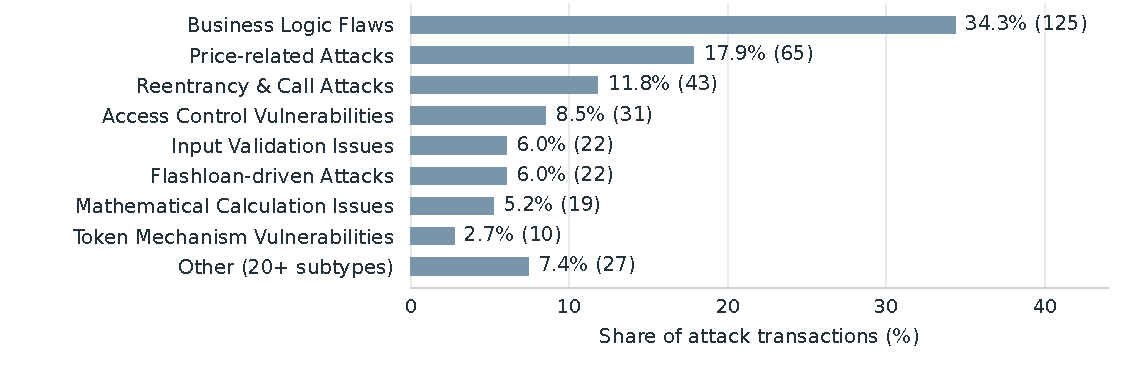
\includegraphics[width=\textwidth]{pic/attack_distribution_bar.pdf}
	\caption{\Blue{Distribution of the 364 attack transactions in \dsystem{}, drawn from DeFiHackLabs. Labels report the percentage and count for each category.}}
	\label{tab:attack_categories}
\end{figure*}

\textit{\textbf{\Blue{Datasets.}}}
\Blue{We use a transaction dataset constructed for this study and a price-manipulation dataset introduced by DeFiScope~\cite{zhong2025detectingvariousdefiprice}.}

\Blue{\textbf{\dsystem{}.} We construct this evaluation set from 364 attack transactions drawn from DeFiHackLabs~\cite{defihacklabs2024}, a public repository of real-world exploit reproductions, and 364 benign transactions sampled from normal user activity in the affected protocols. The benign transactions are selected using temporal proximity to the attacks. We call the resulting balanced set of 728 transactions \dsystem{}. The attack cases span January 2021 to January 2025 and include 110+ labeled exploit types across blockchains such as Ethereum, BSC, and Arbitrum.}
\textcolor{red}{We randomly shuffle the overall transaction collection before partitioning it for model training, knowledge-base construction, and evaluation. The 728 test transactions are disjoint from both the transactions used to train XGBoost and those used to construct the RAG knowledge base.}
\Cref{tab:attack_categories} shows the attack distribution and their proportions.
Business logic flaws and price-related attacks are the most common, accounting for 34.3\% and 17.9\% of the dataset, respectively. Reentrancy and call attacks, access control vulnerabilities, input validation issues, flashloan-driven attacks, mathematical calculation issues, token mechanism vulnerabilities, and other miscellaneous attack types make up the remaining 47.8\%.

\Blue{\textbf{\done{}.} We use the D1 dataset introduced by DeFiScope~\cite{zhong2025detectingvariousdefiprice} for price-manipulation detection. DeFiScope assembled its 95 real-world attacks from DeFort, DeFiHackLabs, and its industry partner, removing duplicate cases across these sources. The attacks caused a reported total loss of \$381.16M on Ethereum and BSC. We could not parse transaction data for four cases and evaluate the remaining 91 attack transactions. We denote this evaluated subset \done{} throughout the paper.}

\textit{\textbf{Baselines.}}
To the best of our knowledge, TrxGNNBERT~\cite{TrxGNNBERT}, TxSpector~\cite{TXSPECTOR}, Blockscan~\cite{wu2025blockscan}, DeFiScope~\cite{zhong2025detectingvariousdefiprice}, DeFort~\cite{defort2024}, DeFiRanger~\cite{defiranger2021}, and DeFiTainter~\cite{defitainter2023} are the most relevant and representative baselines for our evaluation.
Particularly,  TrxGNNBERT~\cite{TrxGNNBERT} powered by a Graph-Transformer architecture, TxSpector~\cite{TXSPECTOR} leveraging static opcode analysis, and Blockscan~\cite{wu2025blockscan} using BERT model enhanced with masked language modeling mechanism, are evaluated on \dsystem{} dataset.
For specialized price manipulation detectors, DeFiScope~\cite{zhong2025detectingvariousdefiprice} combining fine-tuning and pattern learning, DeFort~\cite{defort2024} harnessing symbolic execution and runtime monitoring, and DeFiRanger~\cite{defiranger2021}, and DeFiTainter~\cite{defitainter2023} based on a inter-contract taint analysis, are evaluated on \done{} dataset.
\textcolor{red}{XGBoost-only directly classifies transactions from numerical features. In \approach{}, XGBoost instead guides context selection and prompting, with the LLM producing the final classification. This baseline comparison evaluates direct numerical classification against the combined pipeline.}


\textit{\textbf{Experiment Setup.}}
\RevBlock{LLMs are accessed through third-party APIs. We implement the pipeline with LangChain~\cite{langchain}, Chroma~\cite{chromadb}, and Jina Embeddings v3~\cite{jina2024}. We evaluate nine LLM backbones using the complete pipeline in Figure~\ref{fig:flowchart}; RQ3 compares their detection performance. We treat attacks as the positive class and report accuracy, precision, recall, and F1. A valid prediction is an output that can be parsed as attack or benign, regardless of whether it matches the ground truth. Prediction coverage is the number of valid predictions divided by the total number of test transactions. Accuracy, precision, recall, and F1 are computed on valid predictions; we also report the number of valid outputs.}

\Blue{The XGBoost-only baseline uses 420 training samples and 728 test samples, with balanced attack and benign classes in each set. The tree settings are maximum depth 3, learning rate 0.02, and minimum child weight 1. Row and column subsampling ratios are 0.9 and 0.7; $L_1$ and $L_2$ regularization coefficients are 0 and 0.5.}

\textcolor{red}{We selected the parameter settings empirically based on detection performance in preliminary trials. XGBoost is trained on a balanced set of attack and benign transactions. We use 0.5 as the reference threshold for its probability hint in the LLM prompt, consistent with the equal class proportions in training. A probability below 0.5 prompts closer scrutiny of potential false positives; the LLM makes the final decision based on transaction evidence.}






\subsection{RQ1 (Effectiveness): Comparative Analysis of Detection Accuracy}
To provide a comprehensive assessment of \approach{}'s detection efficacy, we conducted comparative experiments across two datasets with distinct characteristics.
\RevBlock{\approach{} reduces false alarms while maintaining recall close to XGBoost-only (\Cref{tab:performance-dsystem-compact}). It correctly classifies 679 of 728 transactions and achieves 92.93\% F1, compared with 86.48\% for XGBoost-only. Precision rises from 84.33\% to 97.87\%, and false positives fall by 88.33\% (60 to 7), with one additional false negative (41 to 42). XGBoost-only achieves a test AUC of 0.9467. Table~\ref{tab:performance-dsystem-compact} specifies the evaluated samples for each baseline.}

\Blue{The external baselines show different detection trade-offs. Blockscan achieves 95.5\% precision but 70.1\% recall, missing 109 attacks; its F1 is 81.0\%. TrxGNNBERT reports 76.6\% F1, while TxSpector achieves 53.3\% F1 on the 450 transactions it processes. \approach{} combines 97.87\% precision with 88.46\% recall. Relative to Blockscan, this balance corresponds to both fewer false positives (7 versus 12) and fewer missed attacks (42 versus 109).}



\begin{table}[t]
\centering\color{blue}\small
\caption{\Blue{Detection performance on \dsystem{}. \approach{} and XGBoost-only use 364 attack and 364 benign samples. Metrics are percentages.}}
\label{tab:performance-dsystem-compact}
\setlength{\tabcolsep}{2pt}
\begin{tabular}{@{}lrrrrr@{}}
\toprule
Metric & TxSpector & \makecell{TrxGNN\\BERT} & Blockscan & \makecell{XGBoost-\\only} & \approach{}\\
\midrule
$N$ &450&728&728&728&728\\
TP &117&288&255&323&322\\
FP &117&91&12&60&7\\
TN &128&264&352&304&357\\
FN &88&85&109&41&42\\
\midrule
Acc. &54.4&75.9&83.4&86.13&93.27\\
Prec. &50.0&76.0&95.5&84.33&97.87\\
Rec. &57.1&77.3&70.1&88.74&88.46\\
F1 &53.3&76.6&81.0&86.48&92.93\\
\bottomrule
\end{tabular}
\smallskip\par\footnotesize
\RevBlock{$N$ denotes evaluated transactions. TxSpector completes analysis for 450 of 728 transactions; EVM instruction support and runtime limitations account for the remaining 278. Its metrics use the 450 completed analyses. TrxGNNBERT's reported confusion counts correspond to 373 attack and 355 benign transactions.}
\end{table}




\begin{table}[t]
	\centering
	\caption{\Blue{Detection performance on \done{}, the 91-attack subset of DeFiScope\textquotesingle s D1 dataset~\cite{zhong2025detectingvariousdefiprice}.}}
	\label{tab:recall-d1-dataset}
	\small
\setlength{\tabcolsep}{4pt}
	\begin{tabular}{l c c c}
		\toprule
		\text{Tool} &
		\text{\#Attack} &
		\text{Detection Rate} &
		\text{$\Delta$Detection Rate} \\
		\midrule
		DeFort (DF)             & 50  & 54.95\% & $-$25.27\% \\
		DeFiRanger (DR)         & 48  & 52.75\% & $-$27.47\% \\
		DeFiTainter (DT)        & 32  & 35.16\% & $-$45.06\% \\
		DeFiScope (DS)          & 73  & 80.22\% & \textbf{Baseline} \\
		\approach{}   & 86 & 94.51\% & +14.29\% \\
		\bottomrule
	\end{tabular}
\end{table}
\Blue{On \done{}, \approach{} detects 86 of 91 attacks, achieving 94.51\% recall compared with 80.22\% for DeFiScope (Table~\ref{tab:recall-d1-dataset}). The \done{} experiment evaluates specialized price-manipulation detection separately from the \dsystem{} experiment. Table~\ref{tab:ragflow_false_negative} lists the five missed cases.}




\begin{table}[t]
	\centering
	\caption{\Blue{Missed price-manipulation attacks and baselines' detection results.}}
	\label{tab:ragflow_false_negative}
	\small
	\begin{tabular}{l c c c c}
		\toprule
		Attack Case & DS & DT & DF & DR \\
		\midrule
		MerlinLab & \ding{51} & \ding{55} & \ding{55} & \ding{55} \\
		BeltFinance\_1 & \ding{51} & \ding{51} & \ding{55} & \ding{51} \\
		BeltFinance\_2 & \ding{51} & \ding{51} & \ding{55} & \ding{51} \\
		IndexedFinance & \ding{55} & \ding{55} & \ding{55} & \ding{51} \\
		ERC20TokenBank & \ding{51} & \ding{55} & \ding{55} & \ding{51} \\
		\bottomrule
	\end{tabular}
	
	\vspace{0.3em}
	\footnotesize\textit{DS=DeFiScope, DT=DeFiTainter, DF=DeFort, DR=DeFiRanger. \ding{51}=detected, \ding{55}=missed.}
\end{table}

\Blue{The five missed price-manipulation attacks expose challenges in recognizing protocol-specific economic logic and multi-step interactions.}

\RevBlock{The missed cases involve protocol-specific economic behavior. MerlinLab uses a customized oracle update mechanism; BeltFinance involves interactions whose economic effects span multiple steps; IndexedFinance manipulates index-token rebalancing; and ERC20TokenBank exploits internal accounting. These cases require the detector to relate execution steps to protocol-specific pricing or accounting rules, beyond their resemblance to historical traces.}



\begin{tcolorbox}[colback=black!5!white,colframe=black!75!black,sharp corners,fontupper=\small,title=Answer to RQ1]
\Blue{\approach{} achieves 92.93\% F1 and 97.87\% precision. Compared with direct XGBoost classification, it reduces false positives from 60 to 7 with one additional false negative. On \done{}, recall reaches 94.51\%.}
\end{tcolorbox}

\subsection{\Blue{RQ2 (Ablation Study): Effects of Component Configurations}}
\Blue{We fix the default backbone and compare the complete system with three ablated configurations: without XGBoost, without both XGBoost and two-stage retrieval, and without RAG. \textcolor{red}{The no-XGBoost configuration removes numerical risk guidance from context selection and prompting.} The first two ablated configurations yield valid predictions for all 728 transactions. The no-RAG configuration yields 726 valid predictions; its two invalid outputs correspond to attacks.}

\begin{table*}[t]
\centering\color{blue}\small
\caption{\Blue{Component ablation results. Metrics are percentages on valid predictions; counts are ordered TP/FP/TN/FN.}}
\label{tab:ragflow-ablation}
\setlength{\tabcolsep}{3pt}
\begin{tabular}{lrlrrrr}
\toprule
Configuration & $N$ & TP/FP/TN/FN & Acc. & Prec. & Rec. & F1\\
\midrule
Full system &728&322/7/357/42&93.27&97.87&88.46&92.93\\
w/o XGBoost &728&295/98/266/69&77.06&75.06&81.04&77.94\\
w/o XGBoost + two-stage &728&315/110/254/49&78.16&74.12&86.54&79.85\\
w/o RAG &726&278/98/266/84&74.93&73.94&76.80&75.34\\
\bottomrule
\end{tabular}
\smallskip\par\footnotesize
\RevBlock{The w/o XGBoost + two-stage configuration removes both components. No-RAG metrics use 726 valid predictions (99.73\% coverage); the two excluded outputs correspond to attack transactions.}
\end{table*}

\RevBlock{\textbf{XGBoost guidance.} Relative to the no-XGBoost variant, the complete system produces 91 fewer false positives and detects 27 more attacks. These differences correspond to gains of 14.99, 22.81, and 7.42 percentage points in F1, precision, and recall, respectively. In the paired predictions, the complete system correctly classifies 93 benign and 39 attack transactions misclassified by the no-XGBoost variant, but misclassifies two benign and 12 attack transactions that the variant classifies correctly.}

\Blue{\textbf{Two-stage retrieval.} \textcolor{red}{Without XGBoost, F1 is 77.94\% with two-stage retrieval and 79.85\% without it, a decrease of 1.91 percentage points when retrieval filtering is retained.} Its precision is slightly higher (75.06\% versus 74.12\%), but recall is lower (81.04\% versus 86.54\%). \textcolor{red}{The complete system exceeds the variant without both XGBoost and two-stage retrieval by 13.08 percentage points in F1.}}

\Blue{\textbf{No-RAG comparison.} On the 726 transactions with valid predictions in both configurations, the complete system achieves 92.89\% F1, compared with 75.34\% without RAG, a difference of 17.55 percentage points.}

\begin{tcolorbox}[colback=black!5!white,colframe=black!75!black,sharp corners,fontupper=\small,title=Answer to RQ2]
\Blue{The complete configuration improves F1 by 14.99 percentage points over the no-XGBoost configuration and by 17.55 percentage points over the no-RAG configuration on their shared valid samples. Without XGBoost, two-stage retrieval trades higher precision for lower recall and F1.}
\end{tcolorbox}

\begin{figure*}[t]
\centering
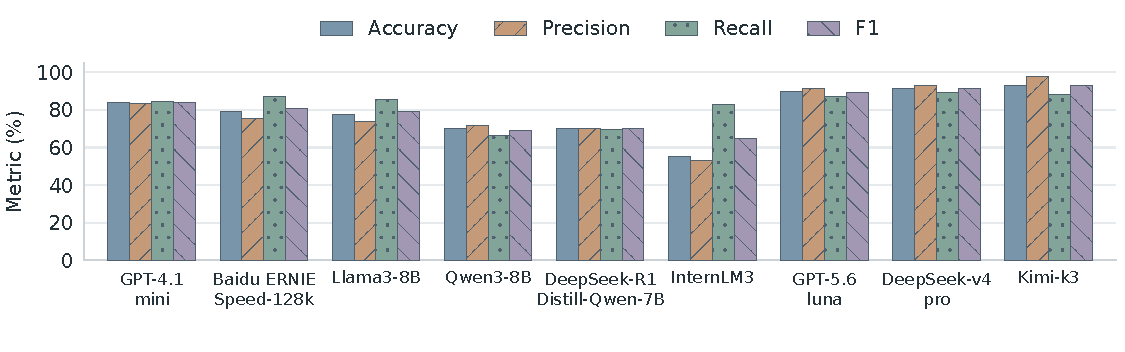
\includegraphics[width=\linewidth]{pic/model_performance_column_chart.pdf}
\caption{\Blue{Detection performance across nine LLM backbones on \dsystem{}. Metrics are percentages.}}
\label{tab:ragflow_results}
\label{fig:backbone_results}
\end{figure*}

\subsection{\Blue{RQ3 (Backbone Ablation): Choice of LLM Backbone}}

\Blue{Figure~\ref{fig:backbone_results} presents the backbone ablation, replacing the default LLM with eight alternatives while retaining the complete \approach{} pipeline. The default backbone achieves the highest precision and F1, with seven false positives, while DeepSeek-v4-pro detects the most attacks. DeepSeek-v4-pro detects 325 attacks compared with 322 for the default backbone, but produces 24 false positives. GPT-5.6-luna detects 318 attacks and produces 29 false positives. Table~\ref{tab:backbone_results} provides the confusion counts and metrics for the default backbone, DeepSeek-v4-pro, and GPT-5.6-luna.}

\Blue{The other backbones exhibit different precision--recall trade-offs within the same pipeline. GPT-4.1-mini achieves 83.9\% F1, with 83.2\% precision and 84.6\% recall. Baidu ERNIE-Speed-128k and Llama3-8B reach higher recall (87.1\% and 85.4\%), but lower precision (75.5\% and 74.1\%), yielding F1 scores of 80.9\% and 79.3\%, respectively.}



\begin{table}[t]
\centering\color{blue}\small
\caption{\Blue{Detailed results for three LLM backbones using the complete \approach{} pipeline ($N=728$ each). Metrics are percentages.}}
\label{tab:backbone_results}
\begin{tabular}{@{}lrrr@{}}
\toprule
Metric & Kimi-k3 & \makecell{DeepSeek-\\v4-pro} & \makecell{GPT-5.6-\\luna}\\
\midrule
TP &322&325&318\\
FP &7&24&29\\
TN &357&340&335\\
FN &42&39&46\\
\midrule
Acc. &93.27&91.35&89.70\\
Prec. &97.87&93.12&91.64\\
Rec. &88.46&89.29&87.36\\
F1 &92.93&91.16&89.45\\
\bottomrule
\end{tabular}
\end{table}

\RevBlock{\textbf{Prediction coverage.} Qwen3-8B produces valid predictions for 588 transactions (80.77\% coverage), with TP=293, FP=97, TN=162, and FN=36. F1 on these valid predictions is 81.50\%; the 140 transactions without valid predictions comprise 35 attacks and 105 benign samples. Table~\ref{tab:noxgb_backbones} reports the backbone ablations without XGBoost and the number of valid predictions for each configuration.}

\begin{table}[t]
\centering\color{blue}\small
\setlength{\tabcolsep}{3pt}
\caption{\Blue{Backbone performance without XGBoost. Metrics are percentages on valid predictions; valid sample counts indicate coverage.}}
\label{tab:noxgb_backbones}
\begin{tabular}{lrrrrr}
\toprule
\makecell[l]{Backbone/\\configuration} & Valid/728 & Acc. & Prec. & Rec. & F1\\
\midrule
BAIDU &727&79.23&75.42&86.81&80.72\\
\makecell[l]{GPT-4.1-mini\\(no RAG)} &728&55.36&80.00&14.29&24.24\\
\makecell[l]{GPT-4.1-mini\\(RAG)} &728&80.91&77.11&87.91&82.16\\
InternLM3 &682&58.80&53.27&94.65&68.18\\
Llama3-8B &726&77.69&73.81&85.64&79.28\\
Qwen3-8B &620&81.94&78.88&83.28&81.02\\
DeepSeek-R1 &682&74.78&70.17&79.87&74.71\\
\bottomrule
\end{tabular}
\end{table}

\begin{tcolorbox}[colback=black!5!white,colframe=black!75!black,sharp corners,fontupper=\small,title=Answer to RQ3]
\Blue{The default backbone provides the highest F1 (92.93\%) and precision (97.87\%) among the nine evaluated backbones, while DeepSeek-v4-pro provides the highest recall (89.29\%). This trade-off allows backbone selection to reflect the relative costs of false alarms and missed attacks.}
\end{tcolorbox}

\subsection{\colorbox{revisionpink}{\parbox[t]{.88\columnwidth}{\color{black}RQ4 (Efficiency): Analysis Latency and API Cost}}}

\RevBlock{We measure per-transaction latency and API cost for the evaluated backbone configurations (Table~\ref{tab:api_cost_comparison}).}



\RevBlock{Table~\ref{tab:api_cost_comparison} reports the latency and API cost of analyzing transaction execution traces. Average end-to-end latency is 15.02 seconds with GPT-4.1-mini, 11.82 seconds with Llama-3.1-8B-Instruct, and 12.66 seconds with Baidu ERNIE-Speed-128k. Retrieval completes in under 100 ms; LLM inference and API communication account for most of the elapsed time. The reported latency covers the complete analysis of each transaction trace.}

\RevBlock{On \done{} (91 transactions), GPT-4.1-mini consumes 5.43 million tokens at a cost of \$2.24, while GPT-3.5-Turbo consumes 5.87 million tokens at a cost of \$3.15. On \dsystem{} (728 transactions), GPT-4.1-mini costs \$3.86 and Llama-3.1-8B-Instruct costs \$0.26 (Table~\ref{tab:api_cost_comparison}).}

To better understand the cost characteristics of different models, we analyzed token consumption during live API evaluation. The results indicate that model-specific verbosity remains a key factor shaping overall token usage. Qwen3-8B produced comparatively longer responses, with outputs reaching up to 29~KB (approximately 7,400 tokens), resulting in a total of 8.15M tokens. InternLM3-8B-Instruct generated more compact outputs, though its total volume (8.2M tokens) remained similar due to retrieval-induced input overhead. DeepSeek-R1-Distill-Qwen-14B exhibited the highest efficiency among the evaluated models, with a total of 7.7M tokens. These observations highlight the combined influence of output verbosity and retrieval context on API-level cost.


While our evaluation primarily focuses on Ethereum and BSC, where most attack cases are currently observed, \approach{} is designed to be extendable to other EVM-compatible blockchains, such as Polygon and Arbitrum. This adaptability ensures that the framework remains applicable as malicious activities evolve and expand across different blockchain ecosystems.

\begin{table}[t]
	\caption{\Blue{Runtime and API cost of \approach{} for the evaluated backbone configurations.}}
	\label{tab:api_cost_comparison}
	\centering
	\small
	\renewcommand{\arraystretch}{1}
	\setlength{\tabcolsep}{1pt}
	\begin{tabular}
		{
		>{\raggedright}p{0.49\columnwidth}
			>{\centering\arraybackslash}p{0.15\columnwidth}
			>{\centering\arraybackslash}p{0.15\columnwidth}
			>{\centering\arraybackslash}p{0.15\columnwidth}}
		\toprule
		\text{Model} & \text{Tokens} & \text{Cost(\$)} & \Blue{Avg. Time (s)}\\
		\midrule
		\multicolumn{4}{l}{\textbf{\done{} (91 samples)}} \\
		\midrule
		GPT-4.1-mini & 5.43M & 2.24 & N/A\\
        \rowcolor{revisionpink} GPT-3.5-Turbo & 5.87M & 3.15 & N/A\\
		\midrule
		\multicolumn{4}{l}{\textbf{\dsystem{} (728 samples)}} \\
		\midrule
		GPT-4.1-mini & 8.62M & 3.86 &  15.02\\
		Llama-3.1-8B-Instruct & 8.28M & 0.26  & 11.82\\
		Baidu ERNIE-Speed-128k & 11.62M & FREE & 12.66\\
		InternLM3-8B-Instruct & 8.2M & FREE & 12.70\\
		DeepSeek-R1-Distill-Qwen-14B & 7.7M & FREE & 32.31\\
		Qwen3-8B & 8.15M & FREE  & 37.54\\
		\bottomrule
	\end{tabular}
	
	\smallskip\scriptsize\textit{Note: Costs are estimated from public API rates; \colorbox{revisionpink}{\parbox{.88\columnwidth}{\color{black}Token counts are total input and output tokens for each evaluated dataset, as reported by the API providers.}}}
\end{table}


\RevBlock{Token consumption, provider pricing, and response latency vary across backbones. The reported costs describe the evaluated API configurations; zero charges reflect the pricing used in these experiments. Deployment choices therefore depend on both detection performance and the available inference service.}

\begin{tcolorbox}[colback=black!5!white, colframe=black!75!black, sharp corners, fontupper=\small, title=Answer to RQ4, label=box:takeaways]
\RevBlock{The evaluated backbones have average per-transaction latencies ranging from 11.82 to 37.54 seconds. For the 728-transaction evaluation, reported API costs range from free access to \$3.86. These measurements quantify the inference overhead of transaction-trace analysis.}
\end{tcolorbox}

\subsection{Discussion: Operational Boundaries and Capability Spectrum}

\RevBlock{Table~\ref{tab:capability_spectrum} summarizes detection rates by attack category. We interpret the differences through three properties: whether the trace exposes discriminative behavior, whether the knowledge base contains analogous attack patterns, and whether identifying malicious intent requires context spanning multiple calls or contracts. These properties help explain where transaction-level reasoning succeeds and where evidence is fragmented or missing.}

We label each category in Table~\ref{tab:capability_spectrum} by the primary bottleneck it presents to \approach{}. \textbf{Low}: high observability and strong analogicality (clear, repetitive trace signatures). \textbf{Medium}: observable core semantics but weaker reusability due to protocol-specific or highly variable logic (analogy-dependent). \textbf{High}: strong contextual dependency, where intent emerges only after aggregating evidence across long, multi-step, or cross-contract execution chains. \textbf{Fundamental}: low observability at the trace-semantic level, where execution remains behaviorally compliant and the malice stems from cryptographic or protocol-assumption violations beyond behavior-only semantics.


\begin{table}[t]
	\centering
	\caption{\Blue{Detection rates in the category-level evaluation.}}
	\label{tab:capability_spectrum}
	\small
\setlength{\tabcolsep}{3pt}
	\begin{tabular}{@{}>{\raggedright\arraybackslash}p{.53\columnwidth}cc@{}}
		\toprule
		\text{Type} & \makecell{Detection\\rate} & \text{Difficulty} \\
		\midrule
		Reentrancy & 96.2\% & Low \\
        Price \& Oracle Manipulation & 93.2\% & Low \\
		Flash-loan Price Manipulation & 91.7\% & Low \\
		Business Logic Flaws & 89.6\% & Medium \\
		Liquidity \& Migration Exploits & 87.5\% & Medium \\
		Arbitrary Call / External Call & 86.7\% & Medium \\
		Access Control & 79.3\% & Medium \\
		Fake Market / MEV / Sandwich Attacks & 75.0\% & High \\
		Signature \& Validation Issues & 57.1\% & High \\
		Cryptographic Exploits  & $<$50\% & Fundamental \\
		\bottomrule
	\end{tabular}
	
	\smallskip\scriptsize\RevBlock{Reentrancy includes two cross-contract cases. Rates describe the category-level evaluation, a separate evaluation from the aggregate backbone results in RQ1--RQ3.}
\end{table}


\approach{} demonstrates its most resilient detection capabilities in scenarios where behavioral anomalies are highly observable and semantic patterns remain stable and reusable. Typical examples include classic reentrancy exploits (96.2\%), flash-loan price manipulations (91.7\%), and price/oracle manipulations (93.2\%). These attacks generate explicit, identifiable signatures within the execution flow, such as the ``unprivileged call to privileged function'' pattern seen in the LocalTrader series, or the ``unexpected state change following an external call'' characteristic of the SpankChain reentrancy exploit. Because the core malicious semantics of these attacks are highly repetitive, \approach{} can leverage its historical case library to establish a robust mapping between ``symptoms'' and ``attack types.'' Consequently, even when encountering novel variants, the system maintains high detection rates through stable pattern matching.

Moving into the domain of common but more sophisticated DeFi exploits---such as Access Control (79.3\%), business logic flaws (89.6\%), arbitrary external calls (86.7\%), liquidity/migration exploits (87.5\%), reflection/token economics flaws, and storage/proxy issues---the system’s performance begins to exhibit fluctuations influenced by the complexity and novelty of the attack patterns. In this domain, \approach{} effectively identifies signatures such as the ``unprivileged call to privileged function'' pattern (e.g., LocalTrader series) or anomalous asset transfer sequences when the knowledge base contains analogous patterns (e.g., Platypus attack). However, performance is challenged by highly innovative or combinatorial variants. For instance, the Indexed Finance exploit utilized a then-novel index token weight rebalancing mechanism; the absence of directly comparable cases in the knowledge base can lead to false negatives. Similarly, variants employing non-standard mechanisms---such as the UwU Lend exploit’s use of median pricing across multiple pools---require the underlying LLM to perform deep reasoning over novel logic rather than simple pattern matching. This area represents a transition for \approach{} from ``pattern matching'' to ``semantic comprehension,'' where accuracy is strictly gated by the breadth of the knowledge base and the model’s reasoning depth.

A more pronounced performance degradation is observed in attacks where malicious intent is decoupled from immediate actions or dispersed across long, complex execution chains. Cross-contract exploits (e.g., Rari Capital, merged into Reentrancy), signature and validation issues (57.1\%), and fake market/MEV/sandwich attacks (75.0\%) exemplify this challenge. The core difficulty lies in the fragmentation of semantic signals: malicious intent is often distributed across multiple contracts or embedded within sequences of seemingly legitimate operations, creating a bottleneck for contextual integration. Intent typically becomes discernible only after aggregating evidence across disparate calls, such as missing \texttt{ecrecover}, replay patterns, MEV ordering, or long-range state effects. Although \approach{}’s retrieval module can surface localized anomalous fragments, its ability to reconstruct a holistic cross-contract call-graph and synthesize these dispersed signals into a coherent attack narrative remains limited, resulting in lower detection rates (approximately 57\%--75\%).


\RevBlock{Cryptographic exploits have detection rates below 50\% in the category-level evaluation. Attacks involving signature malleability or predictable randomness require analysis of the corresponding security assumptions, which may not be explicit in a transaction trace. Numerical errors, such as overflow or precision loss, can similarly require reasoning about expected arithmetic behavior. Combining trace analysis with checks of these properties is a direction for extending detection coverage.}


\RevBlock{Individual incidents also illustrate the diversity of failure mechanisms. DeFiHackLabs documents the February 2024 FILX DN404 incident as an access-control exploit~\cite{defihacklabs_dn404_2024}. The Game exploit combines a bidding-logic flaw with reentrant calls~\cite{defihacklabs_game_2024}, illustrating why analysis may need to connect multiple interacting behaviors within one trace.}

\RevBlock{The category-level results indicate that detection is strongest when execution traces expose recognizable attack behavior. Fragmented cross-contract evidence and attacks without clear behavioral signatures remain difficult. These findings motivate richer call-graph and state-flow representations and complementary analyses for properties that transaction traces alone do not establish.}
